% 图 6.3 顺磁态随机方向自旋 (T>T_C) 与铁磁态一致向上自旋 (T<T_C)
\documentclass[tikz,border=5pt]{standalone}
\usetikzlibrary{arrows.meta}
\usepackage{amsmath}
\usepackage{bm}
\usepackage{fontspec}
\setmainfont{Times New Roman}
\begin{document}
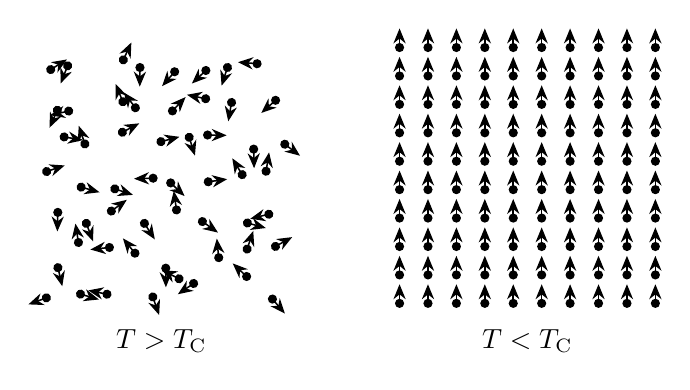
\begin{tikzpicture}[line width=0.8pt,>=Stealth]
\pgfmathsetseed{19650703}
\tikzset{spin/.style={line width=0.55pt,
  {Circle[length=1.15mm,width=1.15mm]}-{Stealth[length=1.9mm,width=1.55mm]}}}
\def\L{3.25}
% ---- left: paramagnetic, random directions (jittered 8x7 grid) ----
\begin{scope}[shift={(0,0.1)}]
  \foreach \i in {0,...,7}{\foreach \j in {0,...,6}{
    \pgfmathsetmacro\x{(\i+0.5)*\L/8+0.16*rand}
    \pgfmathsetmacro\y{(\j+0.5)*\L/7+0.14*rand}
    \pgfmathsetmacro\a{360*rand}
    \draw[spin] (\x,\y) -- ({\x+0.30*cos(\a)},{\y+0.30*sin(\a)});
  }}
  \node at ({\L/2},-0.42) {$T>T_{\mathrm{C}}$};
\end{scope}
% ---- right: ferromagnetic, all up ----
\begin{scope}[shift={(4.65,0.1)}]
  \foreach \i in {0,...,9}{\foreach \j in {0,...,9}{
    \draw[spin] ({\i*0.361},{\j*0.361}) -- ({\i*0.361},{\j*0.361+0.30});
  }}
  \node at (1.6225,-0.42) {$T<T_{\mathrm{C}}$};
\end{scope}
\end{tikzpicture}
\end{document}
